%%
%% This is file `sample-authordraft.tex',
%% generated with the docstrip utility.
%%
%% The original source files were:
%%
%% samples.dtx  (with options: `authordraft')
%% 
%% IMPORTANT NOTICE:
%% 
%% For the copyright see the source file.
%% 
%% Any modified versions of this file must be renamed
%% with new filenames distinct from sample-authordraft.tex.
%% 
%% For distribution of the original source see the terms
%% for copying and modification in the file samples.dtx.
%% 
%% This generated file may be distributed as long as the
%% original source files, as listed above, are part of the
%% same distribution. (The sources need not necessarily be
%% in the same archive or directory.)
%%
%% The first command in your LaTeX source must be the \documentclass command.
% \documentclass[sigconf, review, anonymous, usenames,dvipsnames]{acmart}
\documentclass[sigconf, usenames, dvipsnames]{acmart}


\usepackage{algorithm}
\usepackage{algorithmic}
\usepackage{multirow}
\usepackage{soul}
% \usepackage{balance}
 \usepackage{relsize}
 \usepackage{colortbl}
 \definecolor{paleblue}{RGB}{194,207,237}
 \definecolor{english}{rgb}{0.0, 0.5, 0.0} %wow!! http://latexcolor.com/
 \renewcommand{\labelitemi}{$\mathsmaller{\circ}$}
 \usepackage{mathtools}
\usepackage{etoolbox}
\AtBeginEnvironment{quote}{\singlespacing}


	
\usepackage[english]{babel}
\usepackage{blindtext}
\newcommand{\V}{\mathcal{V}}
\newcommand{\M}{\mathcal{M}}
\newcommand{\Scal}{\mathcal{S}}
\newcommand{\Pro}{\mathrm{Pr}}
\newcommand{\F}{\mathcal{F}}
\renewcommand{\floatpagefraction}{.8}%

    \makeatletter
\def\@fnsymbol#1{\ensuremath{\ifcase#1\or \dagger\or \ddagger\or
   \mathsection\or \mathparagraph\or \|\or **\or \dagger\dagger
   \or \ddagger\ddagger \else\@ctrerr\fi}}
    \makeatother
%%%% As of March 2017, [siggraph] is no longer used. Please use sigconf (above) for SIGGRAPH conferences.

%%%% As of May 2020, [sigchi] and [sigchi-a] are no longer used. Please use sigconf (above) for SIGCHI conferences.

%%%% Proceedings format for SIGPLAN conferences 
% \documentclass[sigplan, anonymous, authordraft]{acmart}

%%%% Proceedings format for conferences using one-column small layout
% \documentclass[acmsmall,authordraft]{acmart}

%%
%% \BibTeX command to typeset BibTeX logo in the docs
\AtBeginDocument{%
  \providecommand\BibTeX{{%
    \normalfont B\kern-0.5em{\scshape i\kern-0.25em b}\kern-0.8em\TeX}}}

%% Rights management information.  This information is sent to you
%% when you complete the rights form.  These commands have SAMPLE
%% values in them; it is your responsibility as an author to replace
%% the commands and values with those provided to you when you
%% complete the rights form.
% \copyrightyear{2021}
% \acmYear{2021}
\setcopyright{rightsretained}
% \acmBooktitle{3rd ACM Conference on Advances in Financial Technologies (AFT '21), September 26--28, 2021, Arlington, VA, USA}
% \acmPrice{15.00}
% \acmDOI{0000000000000000}
% \acmISBN{0000000000000000}
% \acmSubmissionID{5}


%%
%% Submission ID.
%% Use this when submitting an article to a sponsored event. You'll
%% receive a unique submission ID from the organizers
%% of the event, and this ID should be used as the parameter to this command.
%%\acmSubmissionID{123-A56-BU3}

%%
%% The majority of ACM publications use numbered citations and
%% references.  The command \citestyle{authoryear} switches to the
%% "author year" style.
%%
%% If you are preparing content for an event
%% sponsored by ACM SIGGRAPH, you must use the "author year" style of
%% citations and references.
%% Uncommenting
%% the next command will enable that style.
%%\citestyle{acmauthoryear}

%%
%% end of the preamble, start of the body of the document source.

%% comments 
 \newcommand{\dcp}[1]{\textcolor{blue}{{\scriptsize{David:}}#1}}
  \newcommand{\dcpadd}[1]{\textcolor{english}{#1}}
\newcommand{\dan}[1]{\textcolor{DarkOrchid}{{\scriptsize{Dan:}}#1}}
\newcommand{\rithvik}[1]{\textcolor{cyan}{{\scriptsize{Rithvik: }}[[#1]]}}
\newcommand{\rithvikadd}[1]{\textcolor{cyan}{#1}}
\newcommand{\mike}[1]{\textcolor{Maroon}{{\scriptsize{Mike: }}#1}}

\newcommand*{\util}{U_A}
\newcommand*{\reward}{R_A}


\begin{document}

%%
%% The "title" command has an optional parameter,
%% allowing the author to define a "short title" to be used in page headers.
\title{Strategic Liquidity Provision in Uniswap v3}

%%
%% The "author" command and its associated commands are used to define
%% the authors and their affiliations.
%% Of note is the shared affiliation of the first two authors, and the
%% "authornote" and "authornotemark" commands
%% used to denote shared contribution to the research.
\author{Michael Neuder}
\affiliation{%
  \institution{Harvard University}
}
\email{michaelneuder@g.harvard.edu}

\author{Rithvik Rao}
\affiliation{%
  \institution{Harvard University}
  }
\email{rithvikrao@college.harvard.edu}

\author{Daniel J. Moroz}
\affiliation{%
  \institution{Harvard University}
  }
\email{dmoroz@g.harvard.edu}

\author{David C. Parkes}
\affiliation{%
  \institution{Harvard University}
}
\email{parkes@eecs.harvard.edu}

%%
%% By default, the full list of authors will be used in the page
%% headers. Often, this list is too long, and will overlap
%% other information printed in the page headers. This command allows
%% the author to define a more concise list
%% of authors' names for this purpose.
% \renewcommand{\shortauthors}{Neuder, et al.}

%%
%% The abstract is a short summary of the work to be presented in the
%% article.
\begin{abstract}
Uniswap is the largest decentralized exchange for digital currencies. The newest version, called Uniswap v3, allows liquidity providers to allocate liquidity to one or more closed intervals of the price of an asset, instead of over the total range of prices. While the price of the asset remains in that interval, the liquidity provider earns rewards proportionally to the amount of liquidity allocated. This induces the problem of {\em strategic liquidity provision}: smaller intervals result in higher concentration of liquidity and correspondingly larger rewards when the price remains in the interval, but with higher risk. We formalize this problem and study three classes of strategies for liquidity providers: uniform, proportional, and optimal (via a constrained optimization problem). We present experimental results based on the historical price data of Ethereum, which show that simple liquidity provision strategies can yield near-optimal utility and earn over 200x more than Uniswap v2 liquidity provision.
\end{abstract}

%%
%% The code below is generated by the tool at http://dl.acm.org/ccs.cfm.
%% Please copy and paste the code instead of the example below.
%%
\begin{CCSXML}
<ccs2012>
   <concept>
       <concept_id>10010405.10003550</concept_id>
       <concept_desc>Applied computing~Electronic commerce</concept_desc>
       <concept_significance>500</concept_significance>
       </concept>
   <concept>
       <concept_id>10010405.10003550.10003551</concept_id>
       <concept_desc>Applied computing~Digital cash</concept_desc>
       <concept_significance>500</concept_significance>
       </concept>
   <concept>
       <concept_id>10010405.10003550.10003552</concept_id>
       <concept_desc>Applied computing~E-commerce infrastructure</concept_desc>
       <concept_significance>500</concept_significance>
       </concept>
   <concept>
       <concept_id>10010405.10003550.10003557</concept_id>
       <concept_desc>Applied computing~Secure online transactions</concept_desc>
       <concept_significance>500</concept_significance>
       </concept>
   <concept>
       <concept_id>10010405.10003550.10003554</concept_id>
       <concept_desc>Applied computing~Electronic funds transfer</concept_desc>
       <concept_significance>500</concept_significance>
       </concept>
 </ccs2012>
\end{CCSXML}

\ccsdesc[500]{Applied computing~Electronic commerce}
\ccsdesc[500]{Applied computing~Digital cash}
\ccsdesc[500]{Applied computing~E-commerce infrastructure}
\ccsdesc[500]{Applied computing~Secure online transactions}
\ccsdesc[500]{Applied computing~Electronic funds transfer}

%%
%% Keywords. The author(s) should pick words that accurately describe
%% the work being presented. Separate the keywords with commas.
\keywords{blockchain, decentralized finance, Uniswap v3, liquidity provision}

\maketitle

\section{Introduction}\label{sec:intro}
Decentralized finance (DeFi) is a large and rapidly growing collection of projects in the cryptocurrency and blockchain ecosystem. From May 2020 to May 2021, the TVL (total value locked, meaning the sum of all liquidity provided to the protocol) into DeFi protocols ballooned by 100x from 800 million USD to 80 billion USD \cite{defipulse}, beginning with a period of rapid growth in the ``DeFi Summer'' of 2020. DeFi aims to replicate traditional financial intermediaries and instruments using smart contracts executed on blockchains (typically Ethereum). 

Decentralized exchanges (DEXes) allow users to swap tokens of different types without a trusted intermediary. Most DEXes, including Uniswap, fall into the category of {\em constant function market makers} (CFMMs). 
Instead of using an order book as is done in traditional exchanges, CFMMs use an {\em automated market maker} (AMM)  to determine the price of an asset. In {\em Uniswap v2}, token pairs can be swapped for each other using {\em liquidity pools}, which contain both tokens. Permitted trades are determined by the {\em reserve curve}, $x y= k$, where $x$ and $y$ denote the the number of tokens of each type in the liquidity pool, and $k$ remains constant across trades. {\em Liquidity providers} add tokens to liquidity pools for the traders to swap against, and are rewarded through the fees traders pay. An illustrative reserve curve is shown in Figure~\ref{fig:v2v3} (blue). In order to trade some quantity of token $y$ for some quantity of token $x$, the trader must keep the product of reserves constant, i.e., buy $\Delta x$ of $x$ for $\Delta y$ of $y$ such that $(x-\Delta x) (y + \Delta y) = k$.

This reserve curve also defines an effective price for token $x$ in units of token $y$, i.e., $p_x(x,y) = -dy/dx$ \cite{krishnamachari2021dynamic}. In the context of the $xy = k$ curve of Uniswap v2, we have $y=k/x \implies p_x(x,y) = k/x^2$. By convention, we take the ``price" corresponding to the AMM and liquidity pool to be the price of $x$, i.e., $p_x(x,y)$, and we let the $x$ token be volatile relative to the $y$ token.
%
In Uniswap v2, liquidity providers earn rewards when traders use the liquidity to execute swaps, which each incur a constant fee of 0.3\% \cite{adams2020uniswap}. Each liquidity provider provides liquidity on the entire interval of possible prices $(0, \infty)$, and earns rewards based on their fraction of the total liquidity in the pool.\footnote{The end behavior of this derivative demonstrates the support for the range of prices being the interval $(0,\infty)$, with $\lim_{x\to \infty} k/x^2 = 0$, and $\lim_{x\to 0^+} k/x^2 = \infty$.}


On May 3, 2021, Uniswap's new protocol, dubbed {\em Uniswap v3} \cite{adams2021uniswap}, was launched on the Ethereum mainnet. The primary update of Uniswap v3 over Uniswap v2 was the addition of  \textit{concentrated liquidity} \cite{adams2021uniswap}. Within three weeks, the new protocol  accumulated a TVL of over 1.2 billion USD and averaged a daily volume of 1.6 billion USD \cite{univ3_analytics}. 
%
In Uniswap v3, liquidity providers can provide liquidity to each of any number of price intervals, called {\em positions}. Liquidity allocated to position $[p_a,p_b]$ earns rewards from fees when the price remains in that interval. If multiple providers have allocated liquidity over an interval containing the correct price, each is rewarded proportionally to the fraction of the liquidity they own on that price.
%
Figure~\ref{fig:v2v3} (red) demonstrates how the constant product curve of Uniswap v2 is shifted to intercept the axes at $a$ and $b$, which are determined by the upper and lower bound of the price interval of the position. This shifted curve \cite{adams2021uniswap} is given by
\begin{align}\label{eq:v3_curve}
    \left(x + \sqrt{k / p_b} \right) \left(y +\sqrt{k p_a}\right) = k,
\end{align}
and the intercepts, $a$ and $b$ can be calculated by letting $x$ or $y$ equal zero respectively.
%
\begin{figure}
    \centering
    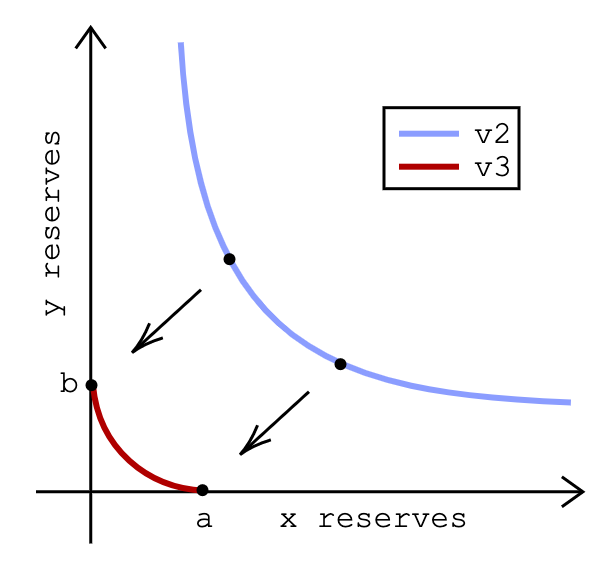
\includegraphics[width=0.5\linewidth]{img/v2v3.png}
    \caption{The reserve curves of Uniswap v2 and v3. Providing concentrated liquidity in v3 on price interval $[p_a,p_b]$ results in shifting the Uniswap v2 curve $xy=k$ to intercept the axes at $a$ and $b$ respectively. The intercepts are calculated by setting $x$ and $y$ equal to zero in the v3 reserve curve (Equation~\ref{eq:v3_curve}).
    \label{fig:v2v3}}
\end{figure}


In this way, Uniswap v3 supports a diversity of strategies in regard to the allocation of  liquidity. Each liquidity provider is presented with a trade off between choosing large positions that cover many possible prices, but earn less fees than smaller, more concentrated positions that are also more risky. 
%dcp edit The liquidity allocation can also be adjusted based on how much risk or variance of rewards that the provider desires.
Additionally, there is a cost of reallocating liquidity, because liquidity allocations are transactions that must be included in a block and thus incur gas fees. This cost must be factored into a liquidity provider's strategy.  

The contributions of this paper are as follows:
\begin{enumerate}
    \item[(1)] formalizing the strategic liquidity provision problem and a family of liquidity provision strategies which we call ``reset liquidity provision strategies'' (reset-LP strategies),
    \item[(2)] presenting three classes of reset-LP strategies for liquidity providers, which we call \textit{uniform}, \textit{proportional}, and \textit{optimal},
    \item[(3)] analytically calculating the expected utility of a reset-LP strategy,
    \item[(4)] solving for the optimal reset-LP strategy based on price-change statistics created from historical Ethereum price data,
    \item[(5)] demonstrating that proportional allocations are optimal for risk-seeking providers and uniform allocations are optimal for risk-averse providers, and
    \item[(6)] back-testing an optimal reset-LP strategy to demonstrate that under suitable conditions, a strategic provider will earn 200x more return on investment than through following a v2 strategy.
\end{enumerate}



% \begin{itemize}
%     \item Rise of DeFi
%     \item Role and history of UniSwap, perhaps pointing to an illustration of v2 vs v3 (the same illustration can be pointed to from the v3 section)
%     \item v3 proposal and timing
%     \item Contribution of this paper
% \end{itemize}

\subsection{Related work}
The Uniswap v1 protocol was defined by \citet{uniswapv1white}, followed up with v2 by \citet{adams2020uniswap}, and most recently amended in v3 by \citet{adams2021uniswap}. 
%

There is a growing body of work studying liquidity provision incentives in Uniswap v2.  
\citet{angeris2019analysis} present an analysis of Uniswap, and more broadly of constant-product AMMs, and demonstrate conditions for which the markets closely track the price on an external reference market. \citet{angeris2020improved} extend this line of research by demonstrating that the more general class of CFMMs incentivize participants to report the true price of an asset on an external market, demonstrating their value as price oracles.

\citet{evans2020liquidity} demonstrates that for {\em  geometric mean market makers} (G3Ms), passive liquidity provision can be used to replicate payoffs of financial derivatives and more active trading strategies. \citet{tassy2020growth} and \citet{uniswapsfinancialalchemy} analyze the growth in wealth of a liquidity provider in CFMM for a geometric Brownian motion price process. \citet{evans2021optimal} extend this to more general liquidity provider objectives and diffusion processes.

\citet{aoyagi2020lazy} study the equilibrium liquidity provision of constant product markets, and show that strategic liquidity providers in the Uniswap v2 environment may have a non-monotonic best response when parameterized with the opponents' liquidity provision. \citet{angeris2020does} extend this line of work to arbitrary CFMMs and calculate bounds on the liquidity provider rewards based on the curve that defines the CFMM.

The above work applies to Uniswap v2 and the general class of CFMMs but not to Uniswap v3. A blog post by \citet{charmalphavault} describes a ``passive rebalancing'' strategy for v3, which aims at maintaining a 50-50 ratio of value for the assets of the liquidity provider. Our work presents a more general class of liquidity provision strategies for Uniswap v3, and introduces a Markov model to evaluate the expected utility of different strategies. To our knowledge, this is the first formal study of  liquidity provision strategies in Uniswap v3.


\subsection{Outline}
Section~\ref{sec:uniswap} introduces the Uniswap v3 protocol and introduces the concept of a liquidity provision strategy. We primarily focus on a class of strategies which we refer to as ``$\tau$-reset'' strategies. Section~\ref{sec:markov} presents the Markov model used to analyze the expected utility of a strategy in this class of strategies. Section~\ref{sec:strats} presents three specific liquidity provision strategies including the optimal $\tau$-reset strategy. Section~\ref{sec:results} presents empirical results based on historical Ethereum price data. Section~\ref{sec:conclusion} suggests open problems for future research and concludes. 

\section{Uniswap v3}
\label{sec:uniswap}

Uniswap v3 introduces to AMMs the concept of \textit{concentrated liquidity}. Instead of providing liquidity on the entire price range of $(0,\infty)$, providers can now specify one or more intervals of price for one of the assets over which to provide liquidity. 
A provider earns transaction fees when the price  of the specified asset is within one of these intervals (and only then). Additionally, if multiple providers allocate liquidity to the same price, they are each rewarded proportionally to the fraction of the total liquidity of that price that they own.

%A rational provider will seek to maximize their expected utility from investment in the reserve pool. 

By choosing more concentrated intervals, a provider can increase their return when the price remains in the interval, but this will also increase the variance in their return. To formalize this, we model a discrete set of price bins, and a provider who chooses how much liquidity to place in each bin and when to reallocate, and who seeks to maximize its expected utility from the stream of fees implied by the adopted strategy.
%
\begin{definition}[Bins]
We define a set of {\em bins} $B = \{b_1, b_2, \ldots, b_c, \ldots\}$, with each bin $b_i$ corresponding to price interval $[l_i,r_i)$, and these form a partition of  $[0, \infty)$, with $l_1=0$ and $r_i=l_{i+1}$ for all $i\in \{ 1, 2, \dots \}$. Bin $b_i$ corresponds to interval $[l_i,r_i)$. Bin $b_c$ denotes the bin containing the {\em current price} of the asset.
\end{definition}

For the remainder of this work we refer to the  price of one asset in a token pair as measured in units of the other. For example, the \texttt{USDC/ETH} pool, where we measure the volatile price of ETH in the stable units of USDC. Consider time $t=n$ and let $P_n$ denote the bin that contains the current price of the volatile asset.
%
A {\em liquidity provision strategy} at time $t=n$ provides a method of determining what proportion of the provider's liquidity  is allocated to each bin.
%
We make the following assumptions:
%
\begin{enumerate}
    \item \textit{Stable price distribution---}We assume the next-price distribution, describing the percent change in price relative to the current price, is constant across time and invariant to the current price. We validated this empirically using the Ethereum 10-minute historical price data, where we found a correlation coefficient of $r^2=0.98$ between the following pairs of probability distributions (i) ETH prices above 300 USD against ETH prices below 300 USD (ii) ETH prices from April 2018-April 2019 against ETH prices from April 2019-April 2020.
    %
    \item \textit{Fixed cost to reallocate liquidity---}We assume that the cost to reallocate the liquidity, which comes from the gas fee of including the associated transaction in a block, is fixed (fixed to $1$), with other values normalized relative to this cost. %dcp edit \footnote{Of course, this choice allows our framework to accommodate, in effect, any constant reallocation cost $c$.} 
    For example if the liquidity provider allocates $\ell=100$ units of liquidity, this is interpreted as 100 times the cost of reallocating  liquidity.%footnote{The cost of reallocating liquidity comes from the gas fee of including a transaction a block.}
    %
    \item \textit{Periodic updates---}We assume that a provider's liquidity allocation is updated periodically, and with an immediate effect of any reallocation. Further, we take the period length to be long enough (at least 10 minutes) that network transmission delay is not a factor, and this is not the focus of this work.
    %
    \item \textit{Single strategic provider---}We assume a single, strategic liquidity provider, and implicitly model the rest of the providers as  allocating liquidity over the entire price range, i.e., following the Uniswap v2 liquidity provision method.
    %dcp edit This allows us to study the optimal allocation for a single-agent. In Section~\ref{sec:future}, we discuss the future work of multi-agent strategic liquidity provision, which is a natural extension to this work.
\end{enumerate}

% In regard to~(2), in reality the fee would depend on the number of bins that liquidity is being allocated to, because bin represents a different position and thus is . Since we consider situations where the provider is providing liquidity on the order of 100x the cost of moving the liquidity, we choose not to model this detail. 

\subsection{Liquidity provision strategies}\label{sec:lpstrat}

In describing the \textit{strategic liquidity provision} problem,
%is defined by (i) a probability distribution over the movement of the price, which we call the %\textit{next-price distribution}, and (ii) the bin containing the current price when the strategy is set, %denoted as $b_s$. 
%
%
we first define the  stochastic process  $\{ P_n : n \in \mathbb{N} \}$ on the price $P_n$  at  time index $n$. 
%
%We model a \dcpadd{time-independent and Markovian} next-price distribution, 
%$\mathrm{Pr}(P_{n+1}=b_i~|~P_n=b_s)$.
%
%induces a probability distribution on the price conditioned on the current price.
%
%
We model a {\em stable} next-price distribution, such that the distribution on next price, describing the change in price relative to the current price, is constant across time and also invariant to the current price.
For this, we re-index the price bins relative to the current price. Let $b_s$ denote the current price bin,  and index this in relative terms as  $b_{(0)}$. Let $b_{(-k)}$ and $b_{(k)}$ denote the $k^{th}$ bin to the left and right $b_{s}$, respectively.
%
The support of the next-price distribution is within set  $B_k = \{-k_{\max}, -k_{\max}+1, \ldots, 0, \ldots, k_{\max}\}$, where $k_{\max}$ is the maximum possible next-price movement.
%
Following Assumption~1, we can write 
%
\begin{align}
    \mathrm{Pr}\left(P_{n+1}=b_{(k)}~|~P_n=b_{(0)}\right)=h(k),  \quad \text{for } k \in B_k,
\end{align}
%
where $h(k)$ is the probability of moving left or right by $k$ bins, depending on the sign of $k$.
%
%dcp edit We assume that this distribution is constant for all $b_{(0)} = b_s \in B$, (e.g., the probability of moving from bin 10 to bin 12 is the same as moving from bin 100 to bin 102), which relies on the stationarity of the next-price distribution (Assumption 1).
% \dcp{anything to say about empirical support for this assumption on ETH, for 10 minute intervals?}.


%\dcp{(1) if you have shorthand for this, e.g., eqn 3 and $f$ then bring it here;
%(2) I think the idea of a ``reset" strategy only makes sense if this is ``homogeneous", i.e., something like $Pr(P_{n+1}=b_{[i]} | P_n=b_{[0]}) = g(i)$ where $_{[1]}, _{[-1]},$ etc notation indicates "1 up from center", "1 down from center" etc and $g(i)$ defines the distribution, with $i$ taking on positive and negative integers;
%(3) you might still want to define the non-homogeneous version first, as in the current eqn 2, I'm not sure; 
%(4)
%I think you may have in mind for your current defn 2.3 LP stragegy, that the allocation function is relative to the center after a re-set, otherwise this whole idea of a ``reset" is not so well motivated... if this is what you intend then the defn needs to work more like  (0) the idea of a center price (the current price at a reset), (1) an allocation $A(i)\in [0,1]$ that specifies the fraction of liquidity allocated to each of bin $i$, where bins are indexed relative to the bin containing the center price, i.e., $i=+1$ is the next highest bin, etc.; (2) the reset condition is also, I think, relative to the center price, i.e., I think you have in mind a set of bins in relative positions to center that trigger a reset... }

%\dcp{I'm worried this above next-price distribution may not be quite what we intend. Don't we have in mind a stationary and ``homogeneous" distribution (not sure this is the right word) such that the price always moves up one bin, up two bins, etc. according to the same distribution, irrespective of $b_c$? this is not captured in the current math }

%\dcp{the rest in the following is a bit informal... can it be made more formal by defining it as a function of price at last reset and current bin? also, consider also constraining the allocation function more, so that it's a ``homogeneous" function of the price at reset; e.g., same shape of investment around the bin containing current price? alternatively, could add this specificity later in the paper, e.g., maybe it doesn't nicely capture ``uniform" as described in example 1 below (I think it could, though, if you imagine current price is 40)}

Given this, we can now define a simple class of liquidity provision strategies.
%
\begin{definition}
A \textit{reset liquidity provision strategy} (reset-LP strategy) is composed of: 
\begin{enumerate}
    \item The bin containing the {\em price at the time of reset}, $b_{s}=b_{(0)}$.
    \item An {\em allocation}, $A(i) \in [0,1]$ that specifies the fraction of liquidity allocated to each bin $b_{(i)}$ in $B_k$.
    \item A {\em reset condition}, which specifies a subset of the bins in $B$ that cause the strategy to reset. Upon a reset, the allocation rule $A$ is used to reallocate liquidity, centered on the new price $b_s$.
\end{enumerate}
%
\end{definition}

% \dcp{I think by tau-reset you might want something stronger, i.e., do you want contiguous, or do you want the same number of bins either side of the center, or do you want the same prob mass in the bins either side of the center, or ... at the moment what you right is kind of what I have in mind for the ``reset condition" in defn 2.3}

%
Of particular interest is the family of $\tau$-reset strategies.
%
\begin{definition}
A {\em $\tau$-reset strategy} is a reset-LP strategy in which the reset condition is defined 
so that there is a reset only when the price is outside the set 
$B_{\tau} = \{b_{(-n_{\tau})}, \cdots, b_{(0)}, \cdots b_{(n_{\tau})}\}$ of $2 n_{\tau} + 1$ of contiguous bins,  centered on  $b_{s}$.
%The number of bins in $B_{\tau}$ is determined by $\tau$ which specifies the amount of centered probability mass contained in $B_{\tau}$ of the next-price distribution relative to the current center. The $\tau$-reset strategy resets once the bin containing the current price, $P_{n}$, is no longer in $B_{\tau}$.
\end{definition}

Sometimes we also use $\tau$ to denote the probability mass of the next-price distribution that is covered by $B_\tau$. For example, if $\tau=0.50$ then $n_\tau$ is selected to be the smallest number such that set $B_\tau$ includes at least 50\% of the next-price probability mass.

\if 0
Note that,
\begin{align}
    B_{\tau} = \{b_{(-n_{\tau})}, \cdots, b_{(0)}, \cdots b_{(n_{\tau})}\}.
\end{align}

\fi

We also sometimes write $B_{\tau}$ to denote the set of relative indices corresponding to this set of bins, i.e., $B_{\tau} = \{-n_{\tau}, \cdots, 0, \cdots n_{\tau}\}$. The usage  will be clear from the context.

% \dcp{the above doesn't define a complete strategy. Is the intent that $S$ also depends on $b_c$ and is stationary across time, i.e., the same strategy is used after each reset?}

\if 0
As a result of the changes introduced in Uniswap v3, liquidity providers now have an infinite number of different strategies to use to provide liquidity. We categorize the sets of strategies into three classes,
\begin{enumerate}
    \item fixed strategies,
    \item moving, constant allocation strategies, and
    \item adaptive strategies.
\end{enumerate}


\subsubsection{Fixed strategies}

\fi

For illustration, consider the following  strategies.

%A fixed strategy is a constant allocation over a range of prices that is not adjusted as the price moves. In Uniswap v2, the only strategy available was fixed and providing liquidity over all price ranges. An example of this type of strategy in v3 is: 

\begin{itemize}
    \item[] Example 1 (Fixed strategy) --- \textit{``Always provide liquidity in the price interval [\$30, \$50].''}
    % \begin{itemize}
    %     \item[] \textit{Allocation:} Divide liquidity evenly among all bins in the interval.
    %     \item[] \textit{Reset:} Never reset.
    % \end{itemize}
\end{itemize}

\begin{itemize}
    \item[] Example 2 (Uniform $\tau$-reset strategy) --- \textit{``Allocate  liquidity uniformly on a range of bins centered on the current price $b_s$. Reset when the price moves outside this range."}
    % \begin{itemize}
    %     \item[] \textit{Allocation:} Divide liquidity evenly among bins interval centered on current price.
    %     \item[] \textit{Reset:} Reset .
    % \end{itemize}
\end{itemize}


\begin{itemize}
    \item[] Example 3 (Proportional $\tau$-reset strategy \#1) --- \textit{``Let $\tau=0.5$, so $B_{\tau}$ contains the middle 50\% of the probability mass of the next-price distribution. Allocate liquidity proportionally to the probability of each bin in $B_{\tau}$. Reset according to $B_\tau$."}
\end{itemize}

\begin{itemize}
    \item[] Example 4 (Proportional $\tau$-reset strategy \#2) --- \textit{``Let $\tau=0.5$, so $B_{\tau}$ contains the middle 50\% of the probability mass of the next-price distribution. Allocate liquidity proportionally to the probability of each bin in the middle 90\% of the probability mass of the next-price distribution. Reset according to $B_\tau$."}
\end{itemize}

%This class of strategies is the easiest to define and analyze. 

%\subsubsection{Moving, constant allocation strategies}\label{sub:classtwo}

\if 0
This class accounts for strategies that have a central bin $b_c$ and a set of bins defined relative to the central bin that liquidity is allocated into. These strategies also have a lower and upper bin, denoted $b_{\min}$ and $b_{\max}$ respectively, past which the liquidity is removed from the previous allocation and reallocated based on a new central bin. The simplest instantiation of this strategy class is:
\begin{itemize}
    \item[] Example 2   --- \textit{``Allocate all of the liquidity the bin containing the current price,and if the price moves, move all the liquidity to the new price.''}
\end{itemize}
In that strategy, the central bin, $b_c$ is the bin of the price at the current time step. Additionally, $b_{\min}=b_{\max}=b_c$, meaning if the price moves outside of that bin, then the strategy will reset to the new price bin. A slightly more complex version of this class if strategies is:
\fi


%In this version, the central bin, $b_c$, is the bin of the price at the current time step, and the provider places liquidity on it and the bins on either side of it. Because the strategy will not be reset until the price leaves this set of three bins, $b_{\min} = b_{c-1}$ and $b_{\max} = b_{c+1}$. 

The uniform $\tau$-reset strategy is illustrated in Figure~\ref{fig:reset_strat}.
%dcp edti This set of examples is by no means exhaustive, and Section~\ref{sec:future} describes potential future work formalizing a more extensive collection. 
%This class of strategies is the main focus of this paper, and we present an analytical method to calculate a probability distribution of outcomes for playing this type of strategy, as well as a method for finding the optimal allocation of liquidity given $b_{\min}$ and $b_{\max}$

% \dcp{I re-purposed your phrasing ``adaptive" to describe a strategy that changes its allocation!}

% \dcp{Need to add additional, illustrative strategies, e.g., proportional allocation, and also suggesting a strategy that may have reset different from allocation range
% in fact, i'd suggest a simple definition of the alpha-tau strategy here}

\if 0

\subsubsection{Adaptive strategies}
This class represents any strategy that not only resets according to the current price, but also may change the allocation of liquidity dynamically based on price dynamics. One implementation of this strategy class is: 
\begin{itemize}
    \item[] Example 4 --- \textit{``Allocate liquidity over a range of bins surrounding the central bin, $b_c$. Reset the strategy once the price leaves the set of bins over which liquidity has been allocated, and choose the window of the new allocation based on the variance of the price movement over the past 12 hours.''}
\end{itemize}
This class encapsulates the most complex strategies, and is presented as a future work opportunity in Section~\ref{sec:future}. For the remainder of this work, we focus on Class 2, which are the moving, constant allocation strategies.

\fi

\begin{figure}
    \centering
    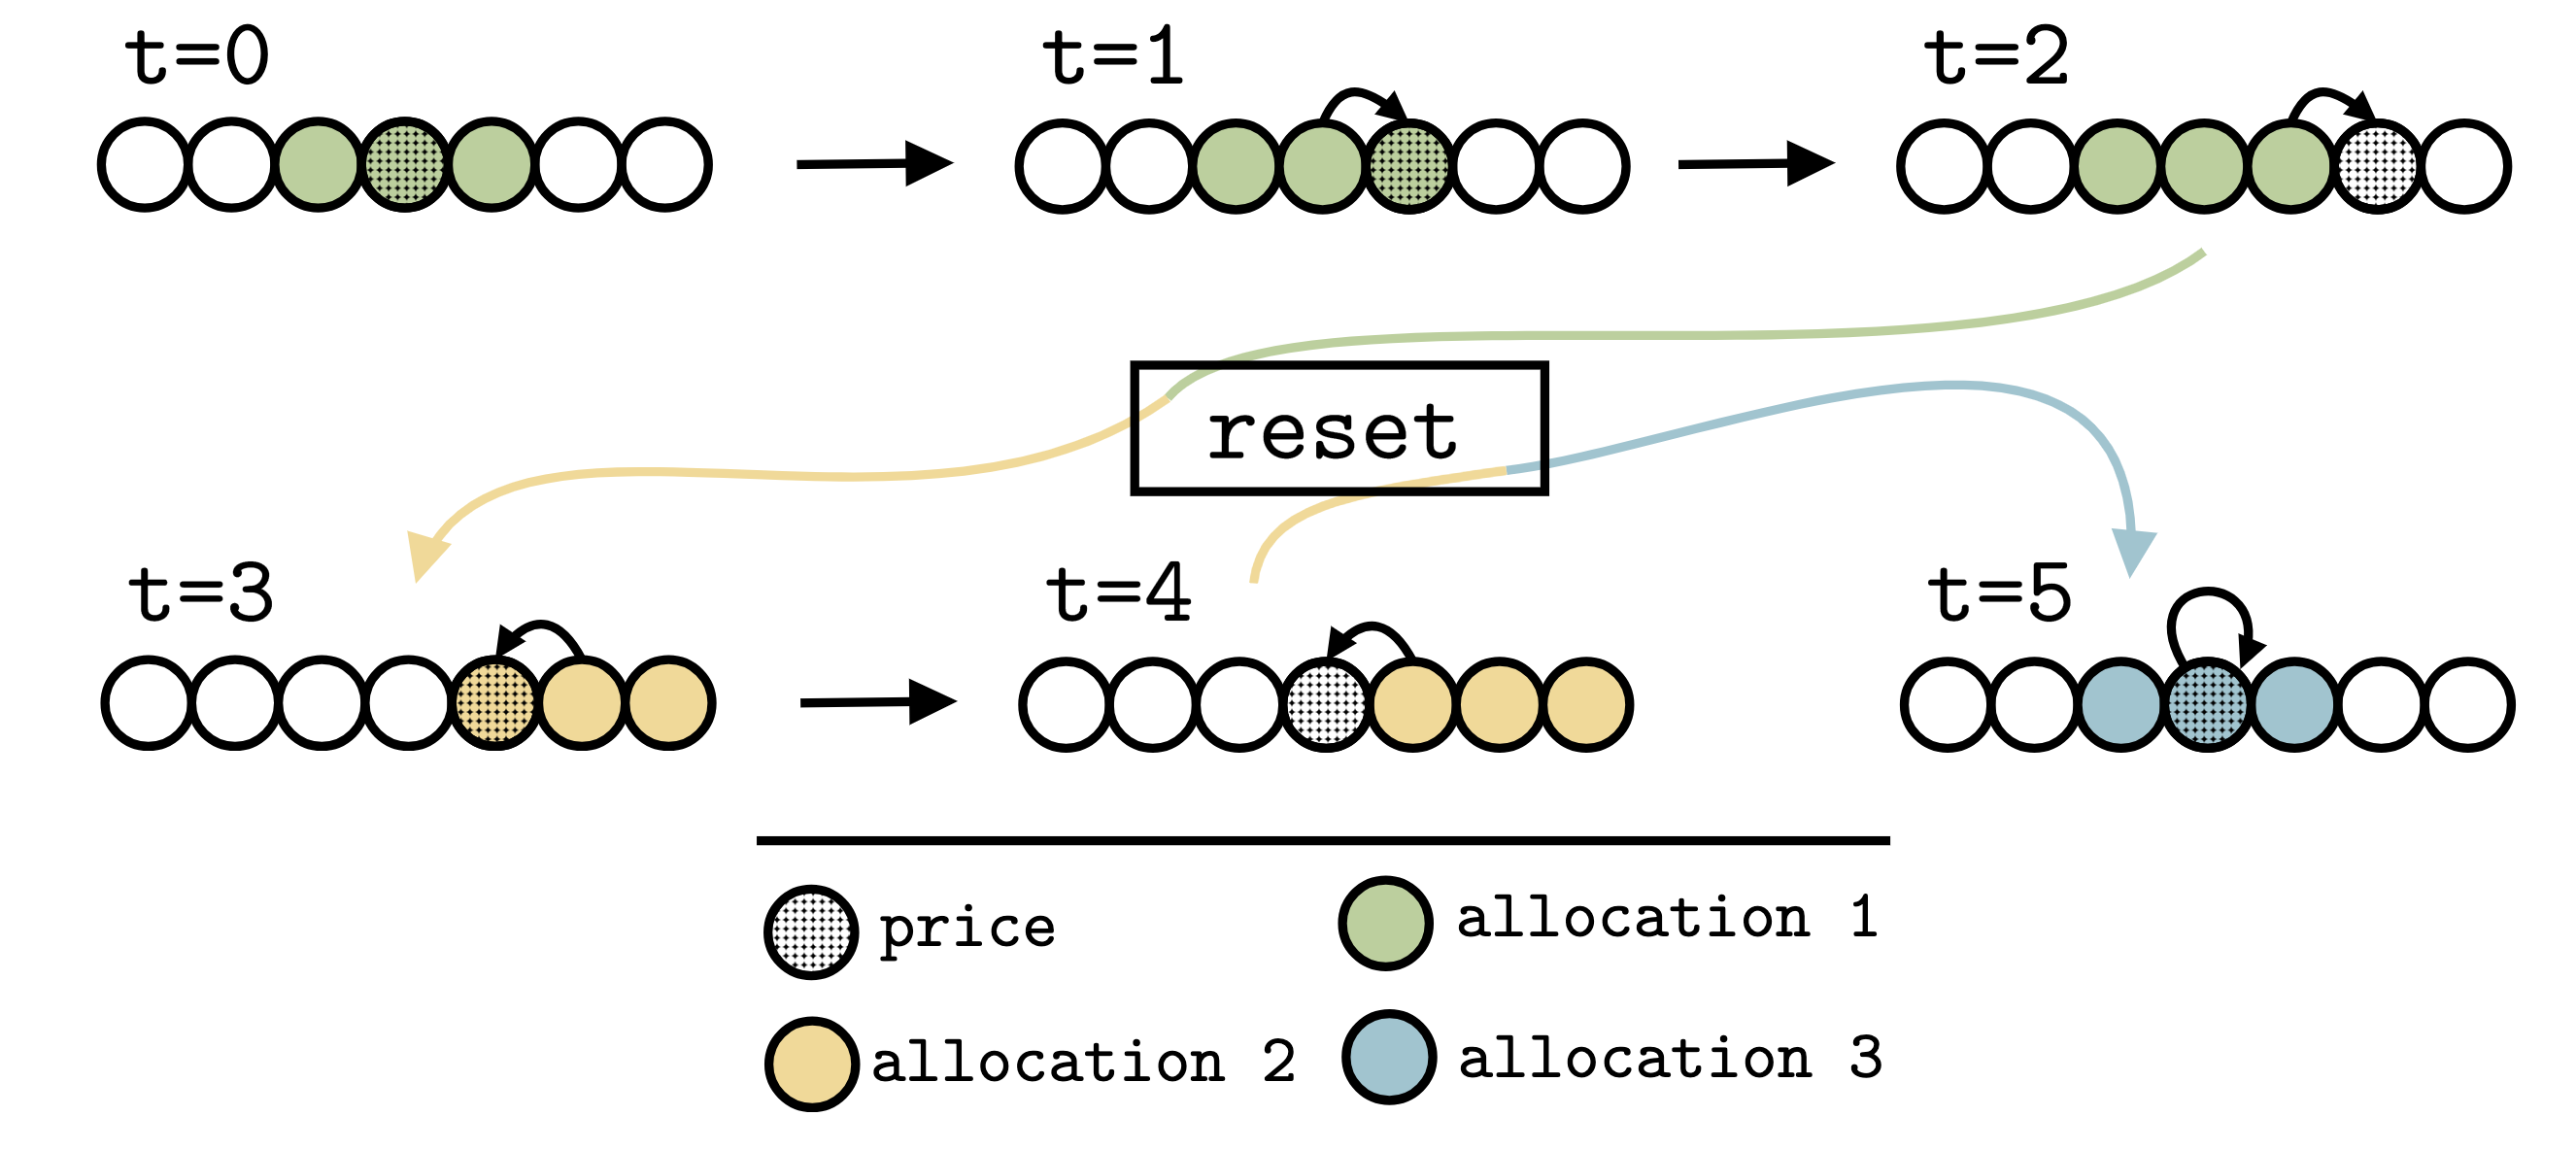
\includegraphics[width=\linewidth]{img/reset_strat.png}
    \caption{The uniform $\tau$-reset strategy, defined here on three contiguous bins centered on the current price.  Each circle represents a price bin, and the darker circle delineates the current price at each time step.
    Once the price leaves these three contiguous bins,  the strategy ``resets" and re-centers the allocation to the price at the time of the reset.
    \label{fig:reset_strat}}
\end{figure}



% \begin{figure}
%     \centering
%     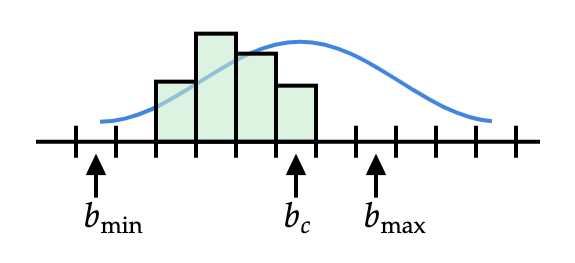
\includegraphics[width=\linewidth]{img/game.png}
%     \caption{A  liquidity provision strategy. Price movements are discretized into bins. The blue line represents the probability distribution of price movements over some amount of time, which we assume is stationary. Shown in green is the liquidity allocated to each bin ($b_c$ is current price, and $b_{\min}$ and $b_{\max}$ denote the range beyond which the provider will ``reset" its allocation). In this case, $B_{\tau}$ is the set of bins from $b_{\min}$ to (and including) $b_{\max}$.
%     \label{fig:game}}
% \end{figure}

\section{Markov analysis}\label{sec:markov}

In this section, We develop an analytical framework with which to determine the expected utility from the fees that flow from a particular reset-LP strategy.

%\dcp{(that said, I'm a bit worried that is not well defined when the current price gets so close to zero that the range of bins cannot be defined in the same way to the left because there aren't enough bins to the left)}

\begin{definition}\label{def:f}
Using relative indices, let $f(i,j) \colon B_{k}\times B_{k} \to [0,1]$ denote the probability of the price moving from the $i^{th}$ bin in $B_{k}$ to the $j^{th}$ bin in $B_{k}$,
\begin{align}
    f(i,j) = \mathrm{Pr}\left(P_{n+1} = b_{(j)}~|~P_n = b_{(i)}\right), \quad \text{for } i,j \in B_k.
\end{align}
Note that $f(i,j) = h(j-i)$, because $h$ defines the probability that the price moves $j-i$ bins.
\end{definition}

Given $P_n = b_{(i)}$, there is also a non-zero probability that the  next price $P_{n+1}$ lands in a bin $b_{(j)} \notin B_{\tau}$. This is the complement of the probability of landing in any of the bins $b_{(j)} \in B_{\tau}$.
%
\begin{definition}
Let $g(i) \colon B_{\tau} \to [0,1]$ denote the probability of resetting, given the price is in the $i^{th}$ bin of $B_{\tau}$,
\begin{align}
    g(i) = 1 - \sum_{j \in B_{\tau}} f(i,j), \quad \text{for } i \in B_{\tau}.
\end{align}
\end{definition}
Landing in a bin outside of $B_{\tau}$ causes a reallocation of liquidity that is centered on $b_s$ (by the definition of the $\tau$-reset strategy), so we can also view a reset as transitioning the price to  the $b_{(0)}$ bin. 

\subsection{Reset Markov chain}

\begin{definition}
The \textit{reset Markov chain}, $M \in \mathbb{R}^{(2n_{\tau}+1) \times (2n_{\tau}+1)}$, where $M(i,j)$ denotes the probability from transitioning to state $j$ given the current state is $i$,  describes the stochastic process of the price movement over the set of bins, $B_{\tau}$, induced by a $\tau$-reset strategy. We have:
\[
M = 
\begin{bmatrix}
  f(-n_{\tau},-n_{\tau}) & \cdots  &f(-n_{\tau}, 0) + g(-n_{\tau}) & \cdots & f(-n_{\tau},n_{\tau}) \\
  \vdots &  & \vdots & & \vdots\\
  f(0,-n_{\tau}) & \cdots  &f(0, 0) + g(0) & \cdots & f(0,n_{\tau}) \\
  \vdots &  & \vdots & & \vdots\\
  f(n_{\tau},-n_{\tau}) & \cdots  &f\left(n_{\tau},0\right) + g(n_{\tau}) & \cdots & f(n_{\tau},n_{\tau}) \\
\end{bmatrix}.
\]
\end{definition}

\begin{definition}
Given $B_{\tau}$, let  $p_{\tau} \in \mathbb{R}^{1 \times (2n_{\tau}+1)}$ denote 
the \textit{stationary distribution} of the reset Markov chain, where
\begin{align}
    p_{\tau} M = p_{\tau}.
\end{align}
\end{definition}

At any  time, the probability that the price is contained within the $i^{th}$ bin of $B_{\tau}$, given a $\tau$-reset strategy, is $p_{\tau}(i)$.


\subsection{Liquidity allocation}

While playing a $\tau$-reset liquidity provision strategy, agents may want to allocate liquidity to a larger set of bins than $B_{\tau}$.
%
\begin{definition}
Let the \textit{$\alpha$ bins}, $B_{\alpha} \subset B$, denote a set of bins $2n_{\alpha}+1$, centered at $b_{(0)}$, over which liquidity is allocated.
\end{definition}

Note that,
\begin{align}
    B_{\alpha} = \{b_{(-n_{\alpha})}, \cdots, b_{(0)}, \cdots, b_{(n_{\alpha})}\}.
\end{align}
Similarly to $B_{\tau}$ we also overload $B_{\alpha}$ to denote the set of relative indices corresponding to this set of bins,
\begin{align}
    B_{\alpha} = \{-n_{\alpha}, \cdots, 0, \cdots, n_{\alpha}\},
\end{align}
and the usage will be clear from context.
%
\begin{definition}
A \textit{liquidity allocation}, $A \colon B_{\alpha} \to [0,1]$, defines the fraction of a provider's liquidity allocated to each bin in $B_\alpha$, and satisfies $\sum_{i \in B_{\alpha}} A(i) \leq 1$.
\end{definition}

In order to evaluate this allocation, for each $j \in B_{\alpha}$, we need (i) the probability of being in  bin $b_{(j)}$ at any given time, and (ii) the utility of being in  bin $b_{(j)}$.
%
\begin{definition}
The \textit{outcome matrix}, $O \in \mathbb{R}^{(2n_{\tau}+1)\times (2n_{\alpha}+1)}$ is,
\begin{align}
O = 
\begin{bmatrix}
  f(-n_{\tau},-n_{\alpha}) & \cdots & f(-n_{\tau}, 0) & \cdots & f(-n_{\tau},n_{\alpha}) \\
  \vdots & & \vdots &  & \vdots \\
  f(0,-n_{\alpha}) & \cdots & f(0, 0) & \cdots & f(0,n_{\alpha}) \\
  \vdots & & \vdots &  & \vdots \\
  f(n_{\tau},-n_{\alpha}) & \cdots & f(n_{\tau}, 0) & \cdots & f(n_{\tau},n_{\alpha}) \\
\end{bmatrix},
\end{align}
which represents the probability of moving from any bin in $B_{\tau}$ to any bin in $B_{\alpha}$.
\end{definition}
The probability of landing in the $j^{th}$ bin of $B_{\alpha}$ 
is calculated by marginalizing out the current location (taking the dot product of the stationary distribution of the Markov chain with each column of the outcome matrix),
%
\begin{align}
    \mathrm{Pr}\left(P_{n+1} = b_{(j)}\right) = \sum_{i \in B_{\tau}} p_{\tau}(i) \cdot f(i,j), \quad \text{for } j \in B_{\alpha}.
\end{align}

To define the utility of each bin in $B_{\alpha}$, we use the  exponential (\textit{constant absolute risk aversion}) utility function \cite{arrow1965aspects, pratt1978risk}.
%
\begin{definition}\label{def:exponential_utility}
Let $u(c)$ denote the exponential utility function,
\begin{align}\label{eq:exponential_utility}
    u(c) &= 
    \begin{cases}
    \left(1-e^{-ac}\right) / a & a\neq 0 \\
    c & a = 0,
    \end{cases}
\end{align}
where $a \in \mathbb{R}$ denotes the Arrow--Pratt measure of absolute risk aversion, a proxy for the provider's degree of risk preference.
% If $a < 0$ the provider is risk-seeking, but if $a > 0$ the provider is risk-averse, and if $a=0$ the provider is risk-neutral. 
Risk-seeking, risk-averse, and risk-neutral preferences correspond to $a < 0$, $a > 0$, and $a = 0$ respectively.
\end{definition}

\begin{definition}
The \textit{reward}, $\reward(j)$, of landing in the $j^{th}$ bin of $B_{\alpha}$ is proportional to the amount of liquidity allocated to that bin. Let $\kappa \in \mathbb{R}^+$ denote the proportionality constant, which is the fraction of the amount of liquidity provided that is earned as a reward in the next time step. From Assumption 4, we assume that $\kappa$ is constant for each central bin $b_s \in B$ and at each time $t=n$.

Additionally, the reward incurs a reset fee of $1$ if the bin is not in $B_{\tau}$, and we have reward function: 
\begin{align}
    \reward(j) =
    \begin{cases}
        \kappa \cdot \ell \cdot A(j) & \text{for } j \in B_{\tau}, j \in B_{\alpha} \\
        \kappa \cdot \ell \cdot A(j) - 1 & \text{for } j \notin B_{\tau}, j \in B_{\alpha}. \\
    \end{cases}
\end{align}
\end{definition}

The utility will depend on the risk preference of the provider. Here,  we increment each reward by one unit, making the  exponential utility function (Equation~\ref{eq:exponential_utility}) well defined (it requires positive inputs). This constant shift does not affect the comparison
of expected utility across different strategies.
%
%, we also need the utility of landing in a bin.
\begin{definition}
The \textit{utility}, $\util(j)$, of landing in the $j^{th}$ bin of $B_{\alpha}$ is
\begin{align}
    \util(j) = u\left(\reward(j)+1\right), \quad \text{for } j \in B_{\alpha}.
\end{align}
\end{definition}

\begin{definition}
The \textit{expected utility}, $E_u$, of an allocation, $A$, is
\begin{align}\label{eq:expected_utility}
    E_u(A) = \sum_{j \in B_{\alpha}}\mathrm{Pr}\left(P_{n+1} = b_{(j)}\right) \cdot \util(j).
\end{align}
\end{definition}

\subsection{Illustrative example}
Consider the simple next-price distribution,
\begin{align*}
    \mathrm{Pr}(P_{n+1}= b_{(-1)}~|~P_n = b_{(0)}) &= 1/3\\
    \mathrm{Pr}(P_{n+1}= b_{(0)}~|~P_n = b_{(0)}) &= 1/3 \\
    \mathrm{Pr}(P_{n+1}= b_{(1)}~|~P_n = b_{(0)}) &= 1/3.
\end{align*}
That is, the price will move down one bin, up one bin, and stay in the same bin, each with probability one-third. This price model is represented in the Markov chain depicted in Figure~\ref{fig:toy_dist}.
\begin{figure}
    \centering
    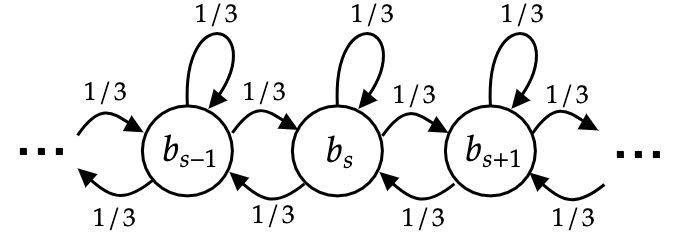
\includegraphics[width=\linewidth]{img/toy_dist.png}
    \caption{The price dynamics in the illustrative example. At each time step, there is a one-third probability of moving left one, moving right one, and staying in the same bin. 
    \label{fig:toy_dist}}
\end{figure}
We use the following $\alpha$ and $\tau$ bins,
\begin{align*}
    B_\tau = B_\alpha&=\{b_{(-1)}, b_{(0)}, b_{(1)}\},
\end{align*}
which also implies that $n_{\alpha} = n_{\tau} = 1$.
We now can calculate the reset Markov chain for the example,
\begin{align*}
    M = 
    \begin{bmatrix}
      1/3 & 2/3 & 0 \\
      1/3 & 1/3 & 1/3 \\
      0 & 2/3 & 1/3
    \end{bmatrix}.
\end{align*}
\begin{figure}
    \centering
    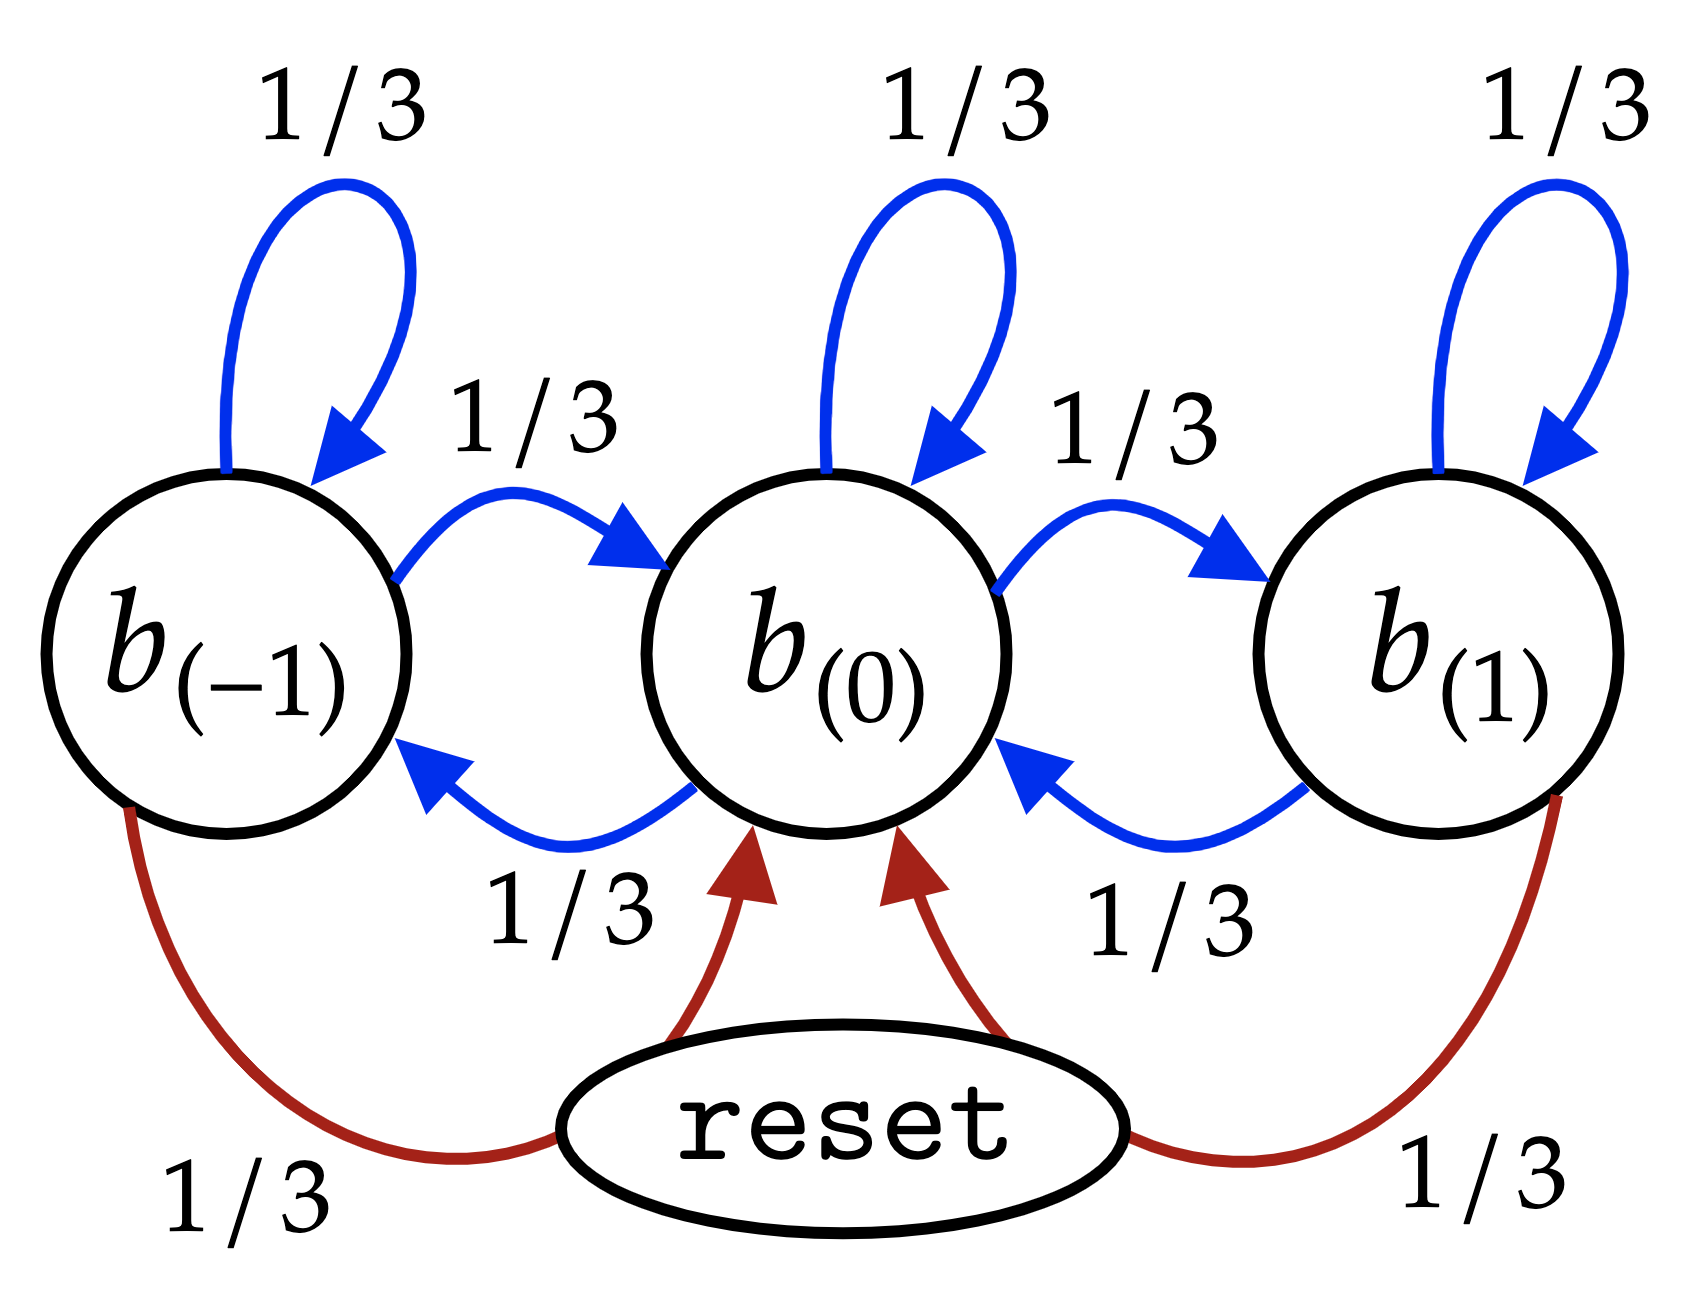
\includegraphics[width=0.7\linewidth]{img/toy_markov.png}
    \caption{The reset Markov chain in the illustrative example.  The center node will move left, right, or stay in the same location with probability one-third, which means it cannot cause a reset, and thus will always earn a reward of $+\kappa \ell /3$. The outer nodes will cause a reset with probability one-third, which will incur a reward of $-1$.
    \label{fig:toy_markov}}
\end{figure}

Figure~\ref{fig:toy_markov} shows this Markov chain visually, where the blue arrows are non-reset transitions, and the red arrows are reset transitions. The stationary distribution of this Markov chain is given by the left eigenvector with eigenvalue 1,
\begin{align*}
    p_{\tau} = 
    \begin{bmatrix}
    1/4 & 1/2 & 1/4
    \end{bmatrix}.
\end{align*}
This means that at any time step, there is a one-half probability that the current price is in the middle bin of the strategy, and there is a one-fourth probability that the current price is in one of the edge bins of the strategy. Let the example allocation be,
\begin{align*}\label{eq:toy_allocation}
    A(j) = 1/3, \quad \textrm{for } j \in B_{\alpha},
\end{align*}
so each bin in $B_{\alpha}$ is allocated one-third of the provider's liquidity. We have the outcome matrix, $O$,
\begin{align*}
    O = 
    \begin{bmatrix}
    1/3 & 1/3 & 0 \\ 
    1/3 & 1/3 & 1/3 \\ 
    0 & 1/3 & 1/3\\
    \end{bmatrix}.
\end{align*}
Let $\ell = \kappa = 1$. By taking the dot product of the stationary distribution, $p_{\tau}$ with each column of the outcome matrix, we calculate the expected utility.
% \vspace{2mm}
% \begin{center}
%     \begin{tabular}{c||c|c}
%     $u$ & $u(1/3)$ & $u(0)$\\
%     \hline
%     $\mathrm{Pr}(U=u)$ & $5/6$ & $1/6$\\
%     \end{tabular}
% \end{center}
% \vspace{2mm}
If we let $a=0$ (risk-neutral), then,
\begin{align*}
    E_u(A) &= 1/3 \cdot 5/6 + 0 \cdot 1/6 \\
    &= 5/18 = 0.2\overline{7}.
\end{align*}
At each time step, we can expect to earn $5/18$ reward for each unit of liquidity that we provide.

% \dcp{I suggest the following }

% \begin{itemize}
%     \item Define the distribution on price changes $f(i,j)$, noting assumed stationary, also introduce the role of $n$ and $n+1$
%     \item Define $B_\tau=\{b_{s-\tau},\ldots,b_s,\ldots,b_{s+\tau}\}$, where I suggest to use $\tau$ in place of your $k$, and we note this is defined in a way that is centered on some bucket $b_s$ . Make clear that $\alpha$ corresponds to when the allocation will be ``reset"
%     \item Define the "reset-MDP", in sense of current Fig 5. 
%     \item Define the transition matrix $M$ for this reset-MDP (I don't think you need to define $M_t$ or $v_r$ explicitly, rather I think you can just define $M$ directly from $f$ and the idea of $1-\sum_j f(i,j)$ for reset probs)
%     \item Define the stationary distribution $p_\tau$ of the reset-MDP
% \end{itemize}

% \dcp{and then the following}

% \begin{itemize}
%     \item Explain that the strategy may invest in a region larger than $\tau$, and that we denote this as buckets $B_\alpha$, allowing for it to be a superset. Don't insist on this being proportional, though
%     \item State we need to compute the utility for being in each of the alpha bins, so that we can get expected utility from $p_\tau$
%     \item Introduce the  exponential utility function
%     \item Try to define utility $v_i$ for some alpha bin $i$ with as minimal notation as possible (I find the current use of $M_o$ a bit complex, and wonder if $v_i$ can be defined more directly in terms of $f$ and $p_\tau$?, without this matrix notation?). ideally the definition of $v_i$ will depend on liquidity allocation $S$, so that it is well defined for different $S$ 
%     \item Somewhere here the role of the rules of uniswap v3 should be clear 
% \end{itemize}


% \dcp{in terms of exposition, try to only use the minimal amount of notation needed, and only use matrices and vectors where helpful, and give a simple  numerical 
% illustration at the end, rather than going through these ``interludes"}

\section{Liquidity Provision Strategies}\label{sec:strats}
We now present three $\tau$-reset strategies.

\subsection{Proportional strategy}\label{sub:prop-adapt}
% \dcp{this section can drop the Markov stuff, but just define the alpha-tau strategy (``proportional-adaptive") precisely. ideally we 
% just consider $\alpha\geq \tau$ and argue that $\alpha<\tau$ is not interesting}
% To demonstrate how to evaluate a liquidity provision strategy, we present a simple strategy called the $\alpha-\tau$, or proportional-adaptive, strategy. 
In this strategy, the provider allocates liquidity proportionally to the probability of landing in a certain $\alpha$ bin. 
% Let $\ell = 100$, where the units are the price of resetting a liquidity provision strategy (the associated gas fees). So the liquidity provider is allocating 100 times the cost of resetting a strategy. 
\begin{definition}
The \textit{proportional strategy} is a $\tau$-reset strategy with:
\begin{enumerate}
    \item The bin, $b_s$,  of  the  price when re-setting the strategy.
    \item The smallest set of consecutive bins, $B_{\tau}$, centered at $b_s$, which account for at least $\tau$ of the probability mass of the next-price distribution. 
    \item The smallest set of consecutive bins, $B_{\alpha}$, centered at $b_s$, which account for at least $\alpha$ of the probability mass of the next-price distribution.
    \item The allocation function
    \begin{align}
        A(j) \propto  h(j), \quad \text{for } j\in B_{\alpha},
    \end{align}
    which allocates all of the liquidity proportionally to the probability of landing in each bin. 
\end{enumerate}
\end{definition}


\begin{figure}
    \centering
    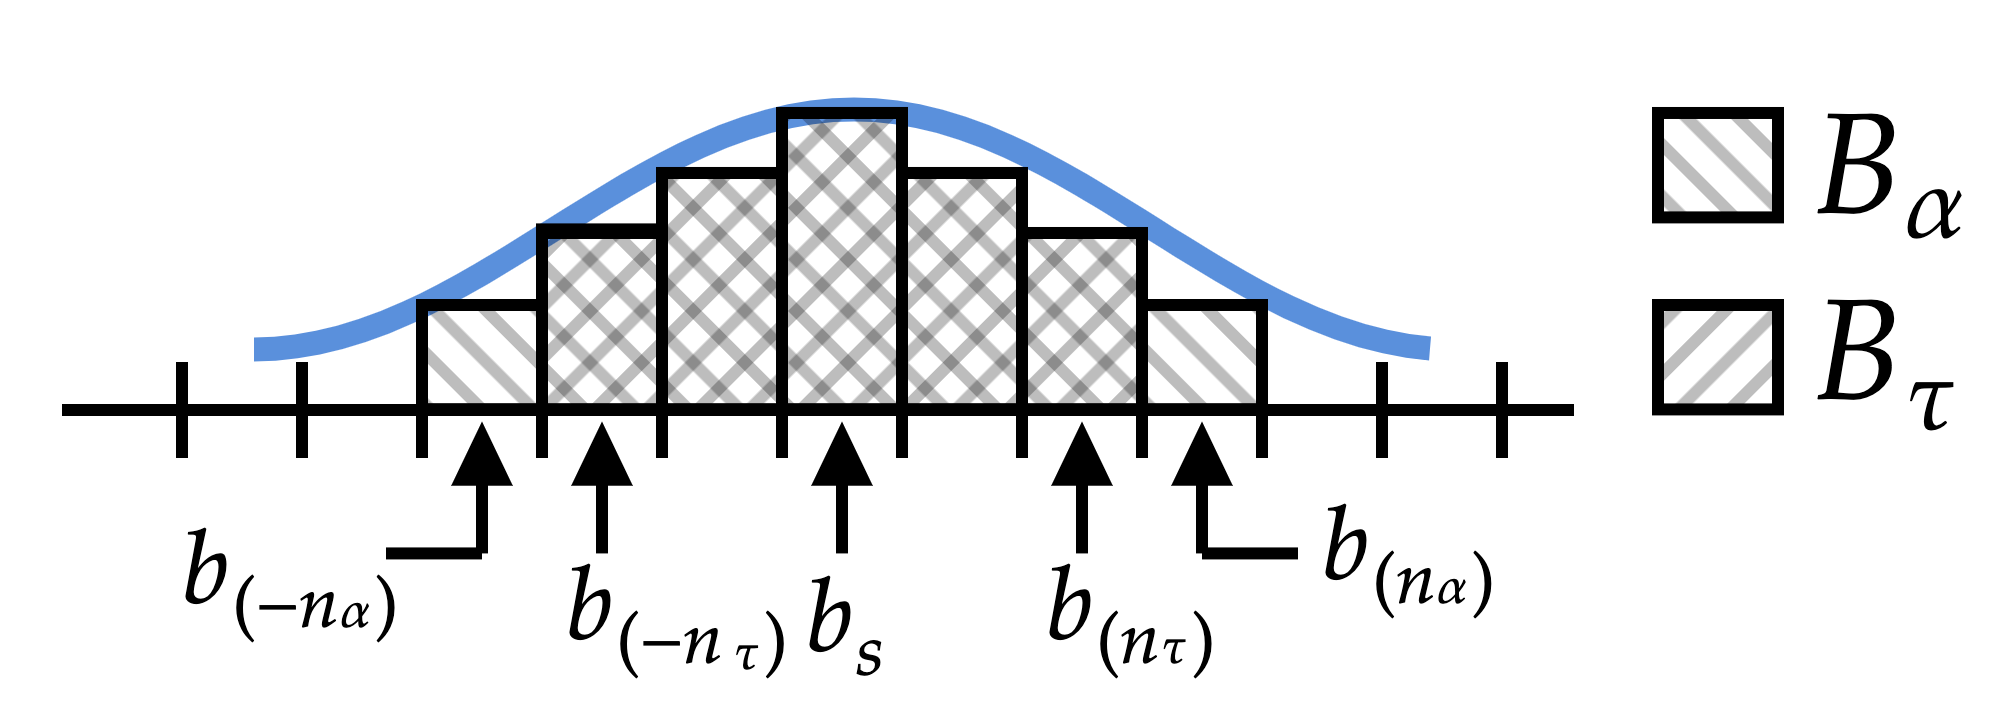
\includegraphics[width=\linewidth]{img/alpha_tau_ex.png}
    \caption{An example of the proportional $\tau$-reset strategy, where $\alpha > \tau$. The height of the bars indicates the amount of liquidity in each bin. When the strategy last reset, the  price was $b_s$. The next-price probability distribution is shown in blue. The ``alpha" and the ``tau" bins are illustrated. In this case, the middle five bins are part of both $B_{\alpha}$ and $B_{\tau}$.
    \label{fig:alpha_tau_ex}}
\end{figure}
Figure~\ref{fig:alpha_tau_ex} shows an example of the proportional strategy, for the case of $\alpha > \tau$. If $\alpha < \tau$, the set of $\tau$ bins would be larger than the set of $\alpha$ bins.

\subsection{Uniform allocation strategy}

In this strategy, the provider allocates liquidity uniformly over the set of $\alpha$ bins. 
\begin{definition}
The \textit{uniform allocation strategy} is a $\tau$-reset strategy with:
\begin{enumerate}
    \item The bin $b_s$ of the price when resetting the strategy.
    \item A set of consecutive bins, $B_{\tau} \subset B$.
    \item A set of consecutive bins, $B_{\alpha} \subset B$.
    \item The allocation function
    \begin{align}\label{eq:at_allocation}
        A(j) = 1 / (2n_{\alpha}+1), \quad \text{for } j\in B_{\alpha},
    \end{align}
    where $n_{\alpha}$ is the number of bins in $B_{\alpha}$.
\end{enumerate}
\end{definition}


\subsection{Optimal liquidity strategy}
In this strategy, the provider allocates liquidity optimally (among $\tau$-reset strategies) over the set of $\alpha$ bins for a specified set of consecutive bins, $B_{\tau}$
%
\begin{definition}
The \textit{optimal liquidity strategy} is defined by:
\begin{enumerate}
    \item The bin $b_s$ of the price when resetting the strategy.
    \item A set of consecutive bins, $B_{\tau} \subset B$.
    \item A set of consecutive bins, $B_{\alpha} \subset B$, defined to  contain every bin that could be transitioned to from a bin in $B_{\tau}$. 
    % \dcp{just $B_k$ now, I think?} not quite, because B_k is the set of bins that can be transitioned to from a single bin, whereas this is from any bin in B_{\tau}
    \item An allocation function, $A$, that is the solution to the liquidity optimization problem, defined as

\begin{equation}
    \begin{aligned}
        \max_{A \in \mathbb{R}^{B_{\alpha}}} \quad& E_u(A) = \sum_{j \in B_{\alpha}} \mathrm{Pr}\left(P_{n+1} = b_{(j)}\right) \cdot \util(j)\\
        \text{s.t.} \quad& \sum_{j \in B_{\alpha}} A(j) = 1 \\
        \quad& A(j) \geq 0 \quad \text{for } j \in B_{\alpha}.
    \end{aligned}
\end{equation}

The constraints specify that (i) all of the liquidity is allocated, and (ii) the liquidity allocated to each bin is non-negative.
\end{enumerate}
\end{definition}

If an interior solution exists, this optimization problem admits a standard solution by way of Lagrange multipliers.
Then the solution is characterized by the system
$$\util'(j) \cdot \mathrm{Pr}\left(P_{n+1} = b_{(j)}\right)  = \util'(k) \cdot\mathrm{Pr}\left(P_{n+1} = b_{(k)}\right) $$
for all $j, k \in B_{\alpha}$, and the constraints
$$\sum_{j \in B_{\alpha}} A(j) = 1$$
and 
$$A(j) \geq 0 \quad \text{for } j \in B_{\alpha}.$$

% Note that the stated solution also gives rise to a heuristic method by which to recover an interior solution: set $A(j) = 0$ for all $j \in B_{\alpha}$, and then iteratively perform gradient ascent until the budget constraint binds.

% \rithvik{should specify what set we are maximizing $A$ over. also should we put in the Lagrangian solution that characterizes the optimizer? this also gives a simple heuristic algorithm to recover the solution}

% \dcp{i'm in favor of both of these changes}

In practice, we solve this constrained optimization problem using the sequential least squares programming (SLSQP) method \cite{boggs1995sequential}. 

\section{Experiments on Historical Ethereum Price Data}
\label{sec:results}


\begin{figure}
    \centering
    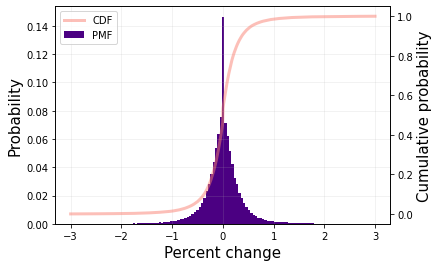
\includegraphics[width=\linewidth]{img/eth_dist.png}
    \caption{The percent-change next-price distribution with 129 bins based on historical Ethereum price data.
    \label{fig:eth_dist}}
\end{figure}

\subsection{Ethereum price data}

To study the liquidity provision strategies described in the previous sections, we create a next-price  distribution from historical Ethereum price data. We use the 10-minute ETH price from March 2018 to April 2020 (100,000 observations). We calculate the percent change in price at every time step, where
\begin{align}
    \text{percent change} = 100 \cdot (P_{n+1} - P_{n}) / P_{n}.
\end{align}
 %\rithvik{should we say something about the (lack of) sensitivity of the analysis to this assumption?}  %dcp I think it's ok not to
%
Figure~\ref{fig:eth_dist} shows the probability distribution of this percent-change next-price ETH distribution, for 129 bins on the interval $[-3\%,3\%]$ with each bin containing about $0.046\%$.
We use this distribution to govern the stochastic process of the price changes for simulating the return on different  liquidity allocation strategies.

% \dcp{anything to say about goodness of stability assumption?}


\subsection{Proportional strategy (Risk neutral provider)}

\begin{figure*}
    \centering
    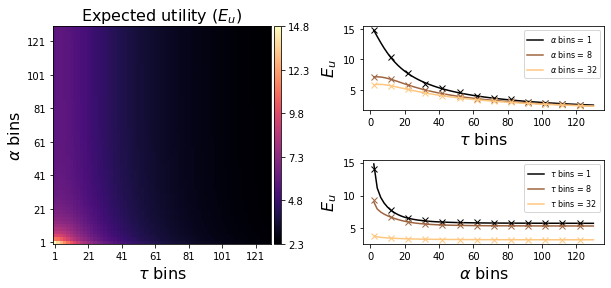
\includegraphics[width=0.8\linewidth]{img/result_sim.png}
    \caption{The expected utility of different proportional strategies for a risk-neutral provider ($a=0$). Left: a density plot of the analytic expected utilities, varying number of $\tau$ bins and $\alpha$ bins. Right: Varying $\tau$ holding number of $\alpha$ bins fixed and varying $\alpha$ holding number of $\tau$ bins fixed. The solid lines denote the results of the analytical, Markov analysis (plugging in the ETH next-price distribution). The $\times$ symbols denote the result of simulating the strategies directly on 50,000 time steps. 
    \label{fig:result_sim}}
\end{figure*}

We first study the expected utility of a risk-neutral liquidity provider ($a=0$) with a proportional allocation strategy for different choices of $\alpha$ and $\tau$, where utility is a function of the expected rewards at each time step given a providers risk preference. 

Figure~\ref{fig:result_sim} (left) shows a density plot of  expected utility.  Figure~\ref{fig:result_sim} (right) shows slices of the surface, first fixing different choices of $n_{\alpha}$ and then fixing different choices of $n_{\tau}$.
We include two different kinds of calculations. The solid lines are based on the analytical results (plugging in the Ethereum next-price distribution to Equation~\ref{eq:expected_utility}). The $\times$ symbols  represent the sample-average utility coming from a direct simulation of the strategy for 50,000 time steps of simulated data. This confirms the validity of the analytical, Markov-chain based model.

For a risk-neutral liquidity provider, the highest expected utility occurs when there is just a single $\alpha$ and $\tau$ bin, i.e., the current bin, $b_s$. In this strategy, the provider allocates all of their liquidity to the single, highest probability bin (which has a probability mass of about $0.15$). Since the provider is allocating 100 units of liquidity, this corresponds to a utility of 15 per time step. 
%, which is why the right hand plots of Figure~\ref{fig:result_sim} max out at about that value. 



% \begin{figure*}
%     \centering
%     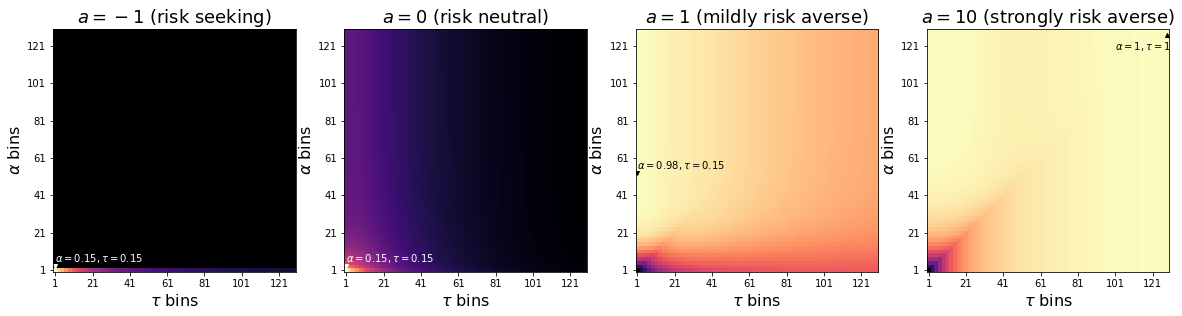
\includegraphics[width=\linewidth]{img/exponential_utility.png}
%     \caption{Expected utility for various levels of risk preference for the proportional allocation strategy. Each of the four axes plots the expected utility on a 2d grid where the $i,j$ element specifies the number of $\alpha$ and $\tau$ bins respectively. Light values are higher expected utilities, and the maximum for each plot is annotated by the text on the figure, which indicates the corresponding values of $\alpha$ and $\tau$ for that proportional strategy.}
%     \label{fig:exponential_utility}
% \end{figure*}


\subsection{Optimal liquidity allocations}


\begin{figure}
    \centering
    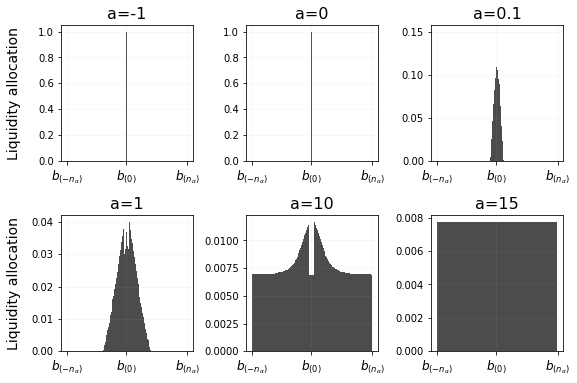
\includegraphics[width=\linewidth]{img/optimal_allocs.png}
    \caption{Optimal distribution for the liquidity allocation of a $\tau$-reset strategy with parameter $n_{\tau}$ set to the smallest value such that $B_\tau$ contains at least 50\% of the probability mass of the next-price distribution. The figure displays the density function of the optimal liquidity allocation. A risk-seeking ($a=-1$) or risk-neutral ($a=0$) provider puts all liquidity into the current-price bin. As the provider becomes more risk averse (e.g., $a=0.1,1,10$), it prefers to use more bins to reduce variance. An  extremely risk-averse provider (e.g., $a=15$) makes a uniform allocation over the $B_\alpha$ bins.
    \label{fig:optimal_allocs}}
\end{figure}


Figure~\ref{fig:optimal_allocs} demonstrates the optimal liquidity allocation for a provider with different levels of risk aversion. This is for a $\tau$-reset strategy with parameter $n_{\tau}$ set to the smallest value such that $B_\tau$ contains at least 50\% of the probability mass of the next-price distribution. For a risk seeking ($a=-1$) or risk neutral ($a=0$) provider, the optimal allocation uses the single, current-price bin. This allocation results in a high expected reward, but a correspondingly high variance. As the provider becomes more risk averse (e.g., $a=0.1,1$), the optimal allocation makes use of more  bins, while still putting a higher proportion of the liquidity into the higher probability, central bins. As the provider becomes very risk averse (e.g., $a=10$), the optimal allocation spreads to cover all bins in $B_{\alpha}$, and for $a=15$ the optimal allocation is  uniform over these bins. 



\subsection{Comparing different strategies}

% Figure~\ref{fig:exponential_utility} shows the expected utilities for various values of risk aversion for the proportional strategy. 

%Using the exponential utility function defined in Definition~\ref{def:exponential_utility}, we can adjust the risk preference ($a$) of a liquidity provider and see the effect on different allocations. 

Figure~\ref{fig:utility_comp} compares performance of the optimal, proportional, and uniform $\tau$-reset strategies for different risk preferences. In each case, we define $n_{\tau}$ as the smallest value such that $B_\tau$ contains at least 50\% of the probability mass of the next-price distribution.

At risk-neutrality ($a=0$) and very low risk-aversion (e.g., $a=0.1$) the proportional strategy is almost optimal with $\alpha=0.14$ and $\alpha=0.74$ respectively. At high levels of risk aversion (e.g., $a=10$), the uniform allocation is near-optimal and for an extremely risk averse provider (e.g., $a=15$), the optimal allocation is exactly uniform. This aligns with the optimal allocations presented in Figure~\ref{fig:optimal_allocs}.

Figure~\ref{fig:opt_tau} demonstrates the optimal expected utility for various values of $\tau$, where $\tau$ defines the proportion of the probability mass of the next-price distribution that the set $B_{\tau}$ contains. For the risk-neutral agent ($a=0$), they prefer small values of $\tau$, because they are willing to update their allocation more frequently given the allocation is all the liquidity in a single bin. For a more risk-averse providers (e.g., $a=3$), they prefer a larger $\tau$ and the resultingly larger number of bins to spread their liquidity over to reduce the variance in the rewards they receive. 



\begin{figure}
    \centering
    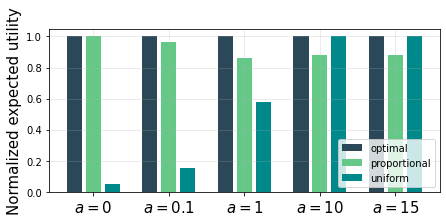
\includegraphics[width=\linewidth]{img/utility_comp.png}
    \caption{Expected utility of the optimal, the best proportional, and the uniform allocation for different risk preferences (values of $a$). For each level of $a$, utility is normalized by the optimal expected utility for that $a$. At lower levels of risk aversion (e.g., $a=0,0.1,1$), the proportional strategy strongly outperforms the uniform allocation. At higher levels of risk aversion (e.g., $a=10,15$) the uniform strategy is optimal. 
    \label{fig:utility_comp}}
\end{figure}

\begin{figure}
    \centering
    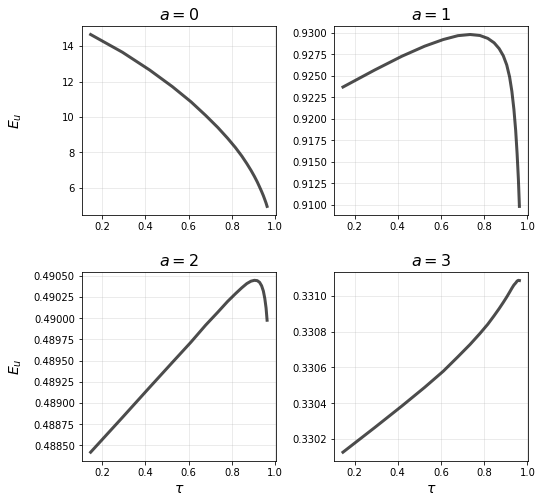
\includegraphics[width=\linewidth]{img/opt_tau.png}
    \caption{Expected utility from the optimal $\tau$-reset strategy as a function of $\tau$. Here, we report  $\tau$ as the amount of probability mass that is contained in the $B_\tau$ bins. A risk-neutral provider ($a=0$) prefers a small $\tau$ and is willing to update its allocation quickly. For a more risk-averse provider (e.g., $a=3$), the opposite is true. Since they are spreading their liquidity over more bins, the optimal $\tau$ is as high as possible to cover more bins and further reduce the variance of their rewards. 
    \label{fig:opt_tau}}
\end{figure}



\subsection{Comparison with Uniswap v2}

Given the historical price data of Ethereum, we can backtest the performance of strategic liquidity provision versus the Uniswap v2 liquidity provision. Recall that in Uniswap v2, liquidity providers aren't able to specify the price intervals over which they want to provide liquidity. 

Figure~\ref{fig:eth_price} shows the historical ETH price for the time period that we use. As denoted in the inset, the black line represents the price of Ethereum at that time period, while the red and blue lines represent the bounds of the $\alpha$ and $\tau$ bins respectively for the optimal $\tau$-reset strategy where $\tau=0.5$ of the next-price distribution and $a=0.1$ (top right allocation of Figure~\ref{fig:optimal_allocs}). This demonstrates how the strategy adjusts the liquidity provision regularly to recenter on the current price. 

To simulate a Uniswap v2 liquidity provision strategy, we  allocate uniformly over the entire price range of the data. In this example, the price ranges from 81 USD to 830 USD, and we discretize this range of prices into about 5500 bins, based on the spacing defined from the empirical calculation of the next-price distribution (Figure~\ref{fig:eth_dist}). 

We allocate liquidity evenly among these 5500 bins, providing a  guaranteed utility of $u(1/5500, a)$ at each time step. We compare this to v3 by finding the optimal $\tau$-reset strategy and dividing the liquidity accordingly to calculate the utility of each price in the data set. The optimal $\tau-$reset liquidity provision strategy has $230x$ more utility than the v2 strategy for the slightly risk averse provider $(a=0.1)$.


\begin{figure*}
    \centering
    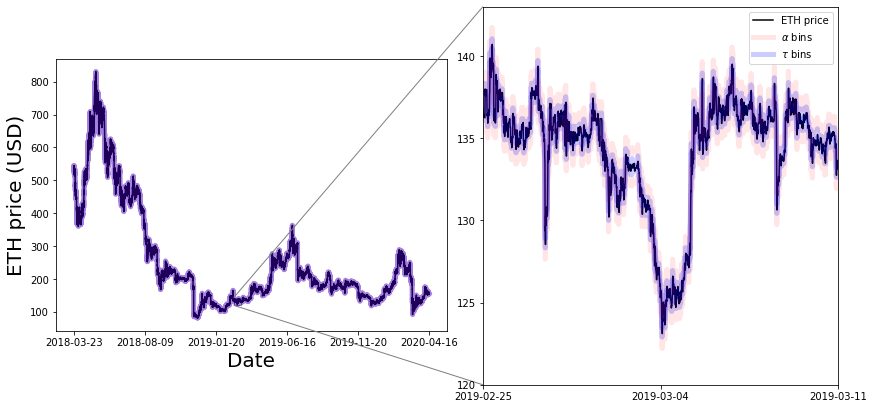
\includegraphics[width=0.7\linewidth]{img/eth_price.png}
    \caption{The optimal $\tau$-reset strategy for $\tau=0.5$ backtested with the historical Ethereum price data. The red lines show the width of the $\alpha$ bins at each time step and the blue lines show the width of the $\tau$ bins. With this strategy, the provider earns on average 230x more utility compared with providing liquidity uniformly across the range of price bins (Uniswap v2 allocation).
    \label{fig:eth_price}}
\end{figure*}

% \begin{figure}
%     \centering
%     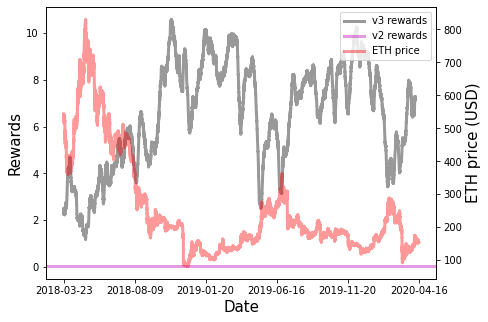
\includegraphics[width=\linewidth]{img/rewards_price.png}
%     \caption{Rewards backtest.}
%     \label{fig:rewards_price}
% \end{figure}

% \blindtext
% \blindtext
% \blindtext
% \blindtext
% \blindtext




\section{Conclusion}\label{sec:conclusion}
This work explores the strategic liquidity provision problem that results from the Uniswap v3 protocol. We present the broad $\tau$-reset class of strategies, and outline a technique for analytically calculating the expected utility of them. We describe three different implementations of the strategy, and compare their performance on the next-price distribution created from the historical Ethereum price data. We are able to find the optimal $\tau$-reset strategy, given a choice of $\tau$ bins, and a next-price distribution. By backtesting our strategy on the historical price data, we find that the optimal $\tau$-reset strategy can have an expected utility that is over 200x the utility a v2 strategy. 


%\subsection{Future work}\label{sec:future}

%As the TVL and trading volume on v3 grow, we expect to see many new strategies emerge. 
%
We hope that this work serves as a first step in formalizing and comparing the performance of these strategies. This present framework only represents a subset of the full strategy space, considering strategies that use the same approach to allocation across time, with the strategy centered on the current price and a reallocation triggered by a large enough price movement. A richer class of strategies would also modify the allocation of liquidity, and reset strategy, based on recent trends in price movement. 

It will be interesting to investigate the question of liquidity provision in a multi-provider context. 
Whereas in this paper we study the investment problem  facing a single v3 player vs a set of v2 players, we see an opportunity in future work to study emergent, equilibrium properties of this Uniswap v3 liquidity provision setting. An empirical study of strategies pursued on Uniswap v3 is also of interest. Additionally, there are intriguing macro-level  connections between Uniswap v3 and gas prices. If gas fees are low, then liquidity providers are motivated to update their positions more frequently, which may cause cause gas prices to rise. Understanding the resulting dynamics and relationship between Uniswap and gas prices is another promising direction.

%% The acknowledgments section is defined using the "acks" environment
%% (and NOT an unnumbered section). This ensures the proper
%% identification of the section in the article metadata, and the
%% consistent spelling of the heading.
\begin{acks}
This work is supported in part by two generous gifts to the Center for Research on Computation and Society at Harvard University, both to support research on applied cryptography and society.
\end{acks}

%%
%% The next two lines define the bibliography style to be used, and
%% the bibliography file.
\bibliographystyle{ACM-Reference-Format}
\bibliography{refs}


\end{document}
\endinput
%%
%% End of file `sample-authordraft.tex'.
